\section{Experimento 3: Consumo Energético en relación al número de cores y threads}
 En este tercer experimento, se ha investigado acerca del consumo energético de procesos de transcodificación ejecutados sobre contenedores de Docker con limitaciones en el acceso a los cores de la CPU y en el número de threads utilizados por los codificadores.

 Para esta subfase experimental se ha utilizado el conjunto de \textit{vídeos} descrito en \ref{tab:exp2.2-videos}, creado y clasificado en el experimento \textbf{Experimento 2.2: Consumo energético en relación al SITI} \ref{section:exp2.2-sitixconsumo}. Del conjunto de vídeos compuesto por un único \textit{chunk}, se han seleccionado dos vídeos correspondientes a cada una de las cuatro zonas definidas en \ref{tab:siti-zones-definition}, obteniendo un total de \textbf{ocho vídeos}, que se muestran en la Tabla \ref{tab:exp2.3-videos-30s}.

 En este caso, se requiere utilizar vídeos de mayor duración que permitan prolongar los procesos de transcodificación, aumentando el tiempo de trabajo de los codificadores y permitiendo recopilar un mayor número de métricas de consumo. Por este motivo, se han generado nuevos vídeos con una duración de \textbf{30 segundos}. Al igual que en la subfase anterior, estos vídeos presentan una resolución de 4K (3840x2160), una tasa de 30 fps y un \textit{bitrate} de 30 Mbps. Para su creación se ha utilizado el \textit{chunk} original, que se ha reproducido en bucle un total de \textit{quince veces}, obteniendo así vídeos con la duración requerida mediante el comando de ffmpeg \lstinline[language=sh,label={code:exp3-ffmpeg-loop-30s}]{ffmpeg -y -stream_loop 15 -i CHUNCKXXX.mp4 -t 30 -b:v 30000k -r 30 -c:v copy -an VIDEO_10S_CHUNCKXXX.mp4}.

\begin{table}[!ht]

 \centering

 \begin{tabularx}{\textwidth}{|X|X|X|X|}

 \hline

 \rowcolor[HTML]{C0C0C0} 

 LSI\_LTI & HSI\_LTI & LSI\_HTI & HSI\_HTI \\ \hline

 LifeUntouched\_0053 & Sintel\_0027 & Eldorado\_0015 & Skateboarding\_0020 \\ \hline

 LifeUntouched\_0056 & TearsOfSteel\_0235 & IndoorSoccer\_0004 & Eldorado\_0010 \\ \hline

 \end{tabularx}

 \caption{Vídeos con una duración de 30 segundos creados para experimentar con el número de threads en relación con el consumo energético}
 \label{tab:exp2.3-videos-30s}

\end{table}

Para llevar a cabo el lanzamiento de los procesos y la recopilación de métricas mediante \textit{Container Energy Monitoring}, se ha desarrollado el script \textbf{exp2.3-threadsxenergy.sh} (Apéndice \ref{code:exp2.3-threadsxenergy}), escrito en Bash. Este script parte de la misma base que el utilizado en la subfase anterior, \textbf{exp2.2-sisti-energy.sh}, pero incorpora determinadas modificaciones para adaptarlo a los nuevos requisitos experimentales. La codificación de los vídeos mostrados en la Tabla \ref{tab:exp2.3-videos-30s} se ha realizado únicamente con los \textit{bitrates} de \textit{10 Mbps} y \textit{30 Mbps} (como se ha definido en la tabla \ref{tab:ana-bitrate-values}), definiendo de esta forma dos escenarios con diferente carga de trabajo y demanda de recursos.

Además, se ha añadido un nuevo nivel de iteración relacionado con el número de cores que el contenedor puede utilizar y con el número de threads que emplea \textit{FFmpeg} durante cada proceso de transcodificación. Para ello, se ha establecido una relación aproximada entre el número de cores disponibles para el contenedor y el número de threads utilizados por \textit{FFmpeg}, expresada como:

\[T_{\text{threads\_FFmpeg}} \approx C_{\text{numero\_cores\_contenedor}}\]

Dado que el sistema utilizado dispone de 8 cores, se ha iterado sobre los valores de \textbf{0, 1, 3, 6 y 7}. Cabe destacar que el valor \textbf{0} representa el escenario sin ninguna restricción en el número de cores ni de threads, utilizándose como referencia para comparar el resto de configuraciones.

Para aplicar estas restricciones, se ha modificado la orden estándar utilizada para ejecutar el proceso de codificación, adaptándola a las características de cada codificador. Utilizando como referencia la información proporcionada en el artículo \cite{threads-number-encoding} y la documentación oficial de los diferentes codificadores \cite{ffmpeg-oficial-documentation} \cite{x265-documentation-threading} se ha llevado a cabo la búsqueda y selección de los parámetros adecuados. Asimismo, mediante el comando \lstinline[language=sh]{ffmpeg -h long encoder=ENCODER} se ha comprobado que las opciones empleadas se encuentran disponibles y son compatibles con la versión de \textit{FFmpeg} instalada. Como resultado, se obtiene la tabla \ref{tab:exp2.3-codecxffpeg-orden-threadlimits}, que recoge las instrucciones utilizadas para limitar el número de threads empleados por cada codificador.

\begin{table}[H]
     \centering
     \begin{tabularx}{\textwidth}{|l|X|}
     \hline
     \rowcolor[HTML]{C0C0C0} 
     \textbf{Codificador} & \textbf{Orden de FFmpeg} \\ \hline
     libx264 & \texttt{ffmpeg -y -i VIDEO-30s.mp4 -c:v libx264 -threads X -b:v [10\textbar 30]M -c:a copy VIDEO-transcoded.mp4} \\ \hline
     libx265 & \texttt{ffmpeg -y -i VIDEO-30s.mp4 -c:v libx265 -x265-params pools=X -b:v [10\textbar 30]M -c:a copy VIDEO-transcoded.mp4} \\ \hline
     H264\_NVENC y HEVC\_NVENC & \texttt{ffmpeg -y -i VIDEO-30s.mp4 -c:v [h264\_nvenc \textbar hevc\_nvenc] -cpucount X -b:v [10\textbar 30]M -c:a copy VIDEO-transcoded.mp4} \\ \hline
     \end{tabularx}
     \caption{Instrucciones de codificación aplicando límites en el número de threads que puede utilizar cada encoder}
     \label{tab:exp2.3-codecxffpeg-orden-threadlimits}

\end{table}

Cabe destacar que, al limitar el número de threads de los codificadores, esta restricción no siempre resulta directamente observable al utilizar herramientas de monitorización como \textit{top} o \textit{htop}. Esto se debe a que la gestión de los threads y de los recursos utilizados durante el proceso de codificación depende del funcionamiento interno de cada codificador, que puede crear y gestionar sus propios threads de manera independiente. Esta característica ha dificultado el proceso de experimentación, ya que la información disponible sobre los mecanismos de control de threads no siempre era suficientemente clara, adecuada para la versión utilizada o se encontraba desactualizada.

Por este motivo, para comprobar que la configuración aplicada producía efectivamente una limitación en el número de threads, se han realizado pruebas individuales con cada codificador, comparando una ejecución con limitación de threads frente a otra sin limitación. Para validar el comportamiento de la configuración, se han utilizado como referencia el tiempo de ejecución y el porcentaje de utilización de CPU obtenidos durante ambas ejecuciones, tal y como se muestra en las Figuras \ref{fig:exp2.3-test-x264-limit-threads} y \ref{fig:exp2.3-test-x265-limit-threads}.

Adicionalmente, en el caso de los codificadores que hacen uso de la GPU, \textit{h264\_nvenc} y \textit{hevc\_nvenc}, no se ha podido establecer una limitación directa sobre el número de threads empleados por el codificador. Únicamente se limita el número de cores de la CPU disponibles para el proceso mediante el parámetro correspondiente, mientras que el propio codificador determina internamente el número de threads adecuado para llevar a cabo la codificación.

Dado que el script está diseñado para poder ejecutarse también en nodos con una mayor capacidad de procesamiento, se ha desarrollado una función denominada \textbf{wake\_up\_containers}, la cual permite crear y arrancar los contenedores aplicando las limitaciones correspondientes en el número de cores. Para ello, tiene en cuenta el número de cores disponibles en el sistema, evitando asignaciones superiores a los recursos existentes que puedan provocar errores de ejecución o un uso inadecuado de los recursos del nodo.

Para llevar a cabo el procesamiento de los datos obtenidos durante los experimentos, se ha desarrollado el script \textbf{ploter-exp2.3.py} (Apéndice \ref{code:exp2.3-ploter} y \ref{code:exp2.3-ploter-obj}). Este script parte de \textbf{ploter-exp2.2.py} como base, pero incorpora modificaciones tanto en el procesamiento de los datos como en las gráficas generadas. Al igual que en la subfase anterior, los resultados se procesan a partir de archivos CSV. Sin embargo, en esta ocasión se incorpora el tiempo necesario para completar cada proceso de transcodificación y se descartan las características SI, TI y la zona a la que pertenece cada vídeo, ya que el objetivo principal de esta subfase es analizar la relación entre el consumo energético, el tiempo de codificación y la disponibilidad de recursos computacionales. La estructura de la cabecera del archivo CSV resultante puede observarse en la Figura \ref{img:exp2.3-csvheader-process-data}.

\begin{figure}[H]
    \centering
    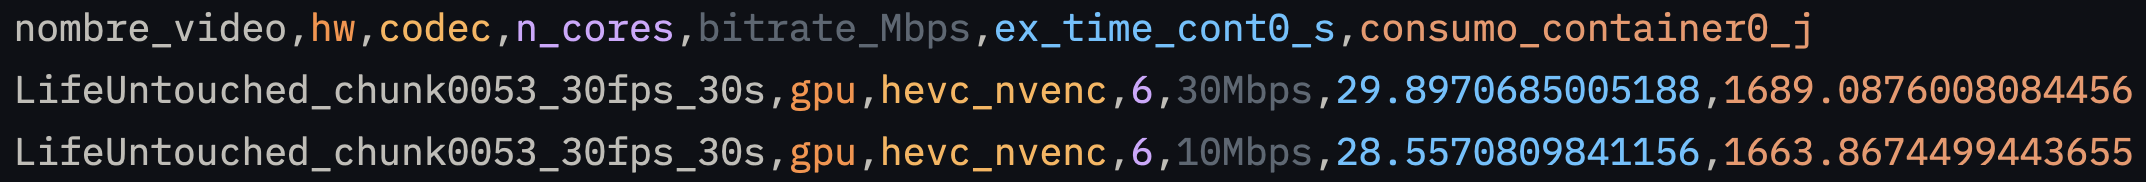
\includegraphics[width=\linewidth]{figs/exp2.3-csvheader-process-data.png}
    \caption{Header CSV del archivo de datos procesados con el script exp2.3-threadsxenergy.sh}
    \label{img:exp2.3-csvheader-process-data}
\end{figure}

El funcionamiento del script es similar al empleado en la subfase anterior. Su ejecución se realiza mediante línea de comandos, indicando el nombre del experimento y, mediante diferentes \textit{flags}, las operaciones que se desean realizar. La ejecución básica del script \textbf{ploter-exp2.3.py} es \lstinline[language=sh]{python3 ploter-exp2.3.py NOMBRE-EXPERIMENTO [FLAGS]}. A continuación, se describen las principales opciones disponibles y el conjunto de gráficas que es capaz de generar:

\begin{itemize}

 \item \textbf{process:} Procesa los datos de las métricas ubicadas en \lstinline[language=sh]{exp2.3-limited_cores_threads/metricas/nombre-experimento} y genera un archivo CSV con los resultados procesados, que se almacena por defecto en \textit{\$(pwd)/data/exp2.3\_process\_data.csv}.
 \item \textbf{plot-consumoxcores:} Genera gráficas que representan el consumo energético (eje Y) en función del número de cores (eje X). Se genera una gráfica para cada proceso de codificación, considerando un codificador y un \textit{bitrate} determinado. Estas gráficas permiten analizar, por una parte, el comportamiento de cada codificador frente a las diferentes restricciones de recursos y, por otra, las diferencias existentes entre los vídeos con distintas características de SI y TI.
 \item \textbf{plot-consumoxcores-gpuvscpu:} Genera grupos de gráficas en los que se representa el consumo energético (eje Y) en función del número de cores (eje X). Cada gráfica muestra el consumo energético de un vídeo codificado empleando un estándar determinado mediante CPU y su equivalente mediante GPU (implementación \textit{libx264} frente a \textit{h264\_nvenc} y \textit{libx265} frente a \textit{hevc\_nvenc}), agrupando los resultados según el \textit{bitrate} utilizado durante la codificación. El objetivo es analizar la eficiencia energética de la utilización combinada de CPU y GPU frente al uso exclusivo de CPU durante el proceso de transcodificación.
 \item \textbf{plot-tiempoxcores:} Genera gráficas lineales agrupadas por nombre del vídeo, \textit{bitrate} y estándar del codificador (implementación \textit{x264} frente a \textit{H.264} o \textit{x265} frente a \textit{HEVC}). En estas gráficas se representa el tiempo de codificación en el eje Y frente al número de cores empleados durante el proceso en el eje X. El objetivo es analizar cómo varía el tiempo necesario para completar el proceso de codificación en función de los recursos computacionales disponibles, permitiendo comparar el comportamiento de los diferentes codificadores al modificar el número de cores y threads utilizados.
 \item \textbf{plot-consumoxtiempo:} Genera un conjunto de gráficas de puntos agrupadas por nombre del vídeo, estándar del codificador (implementación \textit{x264} frente a \textit{H.264} o \textit{x265} frente a \textit{HEVC}) y \textit{bitrate}. En estas gráficas se representa el consumo energético en el eje X frente al tiempo necesario para completar la codificación en el eje Y. Cada gráfica contiene dos grupos de puntos, correspondientes respectivamente al codificador basado en CPU y a su equivalente basado en GPU. Además, cada punto se identifica mediante el número de cores empleados durante la codificación. El objetivo es comparar la eficiencia de los diferentes codificadores en términos de tiempo de ejecución y consumo energético, teniendo en cuenta la cantidad de recursos computacionales utilizados.
 \item \textbf{plot-consumoxtiempo-group:} Permite obtener una gráfica de dispersión de puntos, en la cual se compara el consumo energético (y) frente al tiempo de codificación. Las gráficas se agrupan por bitrate empleado, codificador y número de cores/threads del proceso. Permite establecer y visualizar cómo reacciona cada video del data set a la limitación de cores y threads, así como el grupo de características SITI en el que se encuentra cada uno de estos videos.
 \item \textbf{--data-results:} Permite definir el directorio en el que se almacenan los resultados del procesamiento. Por defecto, su valor es \textit{\$(pwd)/data/exp2.3\_process\_data.csv}.
 \item \textbf{--data-path:} Permite definir la ruta en la que se encuentran las métricas que se desean procesar. Por defecto, tiene el valor \textit{/exp2.3-limited\_cores\_threads/metricas/name-experiment}.

\end{itemize}

\subsection{Resultados del Experimento 3: Consumo Energético en relación al número de cores y threads}
 Las gráficas que se presentan en esta sección han sido generadas mediante el script \textbf{ploter-exp2.3.py} (Apéndice \ref{code:exp2.3-ploter}), y al igual que en el subapartado de conclusiones del experimento 2, se ha reubicado el conjunto de gráficas a la sección \textbf{Experimento 3: Consumo Energético en relación al número de threads y cores} \ref{apendice:exp2.3-graficas}. Únicamente se han incluido las gráficas visibles en la Figura \ref{fig:result-exp3} como muestra de los tipos de gráficas generadas en este apartado experimental.
 
 Los resultados obtenidos permiten confirmar parcialmente la segunda hipótesis de investigación, planteada en el subapartado \textbf{Hipótesis Iniciales} \ref{subsec:hipotesis}, relativa a la influencia del número de \textit{cores} sobre el consumo energético. El comportamiento observado depende en gran medida del codificador utilizado y de las características del vídeo procesado. En particular, la reducción del número de \textit{cores} disponibles tiene un efecto significativo sobre el tiempo de ejecución, aunque disponer de un mayor número de \textit{cores} no implica necesariamente una reducción proporcional del consumo energético. Por tanto, el incremento de los recursos de procesamiento puede proporcionar mejoras considerables en el tiempo de codificación, pero estas mejoras no siempre se traducen en una mayor eficiencia energética. Este aspecto resulta especialmente relevante desde el punto de vista del aprovechamiento de los recursos disponibles, ya que una configuración que minimice el tiempo de ejecución no tiene por qué ser la que presente el menor consumo energético.
 
 En primer lugar, el análisis del consumo energético muestra que el \textit{bitrate} empleado durante la codificación influye de forma directa sobre el comportamiento energético de las cargas de trabajo. En general, los procesos realizados con un \textit{bitrate} de \textit{30 Mbps} presentan consumos superiores a los realizados con \textit{10 Mbps}. Esta diferencia también se refleja en el tiempo necesario para completar la codificación, especialmente en los codificadores basados en CPU, donde se observan diferencias más pronunciadas entre ambas configuraciones.

 \begin{figure}[H]
   \dosubfigs
        {figs/exp2.3/ploter2.3/consumoxcores/libx264-30Mbps_ConsumoxCores.png}{Grafica comparativa de consumo energético frente a número de cores codificador con libx264 y 30 Mbps de bitrate}{fig:result-exp3.2-consumoxcores-x264-30mbps}
        {figs/exp2.3/ploter2.3/tiempoxcores/Eldorado_chunk0010_30fps_30s-10Mbps_libx264_libx265_TiempoxCores.png}{Grafica comparativa de tiempo de codificación frente a número de cores codificado con libx264 y libx265 a 30 Mbps de bitrate para el video Eldorado\_chunk0010}{fig:result-exp3.2-tiempoxcores-x264-30mbps}

   \dosubfigs
        {figs/exp2.3/ploter2.3/consumoxtiempo/Eldorado_chunk0010_30fps_30s-10Mbps_libx264_libx265_ConsumoxTiempo.png}{Grafica comparativa de tiempo de codificación frente a número de cores codificador con libx264 y libx265 a  30 Mbps de bitrate para el video Eldorado\_chunk0010}{fig:result-exp3.2-tiempoxconsumo-x264-30mbps}
        {figs/exp2.3/ploter2.3/consumoxtiempo-group/30Mbps/cores_8/hevc_nvenc-30Mbps_8_ConsumoxTiempoGroup.png}{Grafica comparativa de consumo energético frente a tiempo de codificación con libx264 a 30 Mbps y 8 cores, para todos los videos del dataset}{fig:result-exp3.2-tiempoxconsumo-x264-30mbps-8nucleos}
   \caption{Muestra de los tipos de gráficas obtenidas en el Experimento 3}
   \label{fig:result-exp3}
 \end{figure}

 En el caso de \textbf{libx264}, los resultados muestran una tendencia general hacia la reducción del consumo energético a medida que aumenta el número de \textit{cores} disponibles, acompañada de una disminución del tiempo necesario para completar la codificación. Sin embargo, a partir de \textit{6 cores}, el incremento de recursos proporciona beneficios reducidos. En este punto, las configuraciones superiores no aportan reducciones adicionales del consumo superiores al \textit{7--8\%} y se observa también un cierto estancamiento en el tiempo de ejecución, con reducciones inferiores al \textit{15--18\%}. Estos resultados sugieren que, para las cargas analizadas con \textit{libx264}, la incorporación de recursos adicionales resulta progresivamente menos eficiente a partir de \textit{6 cores}. Por tanto, esta configuración podría considerarse un punto de equilibrio entre consumo energético y tiempo de ejecución para el conjunto de muestras estudiado.

 No obstante, esta tendencia no se presenta con la misma intensidad en todas las muestras, por lo que no puede considerarse un comportamiento generalizable a cualquier carga de codificación. Sería necesario ampliar el estudio utilizando una CPU con un mayor número de \textit{cores} y un conjunto de vídeos más amplio y representativo de diferentes regiones del espacio definido por las características SI y TI para determinar con mayor precisión el punto de saturación de \textit{libx264}.

 En el caso de \textbf{libx265}, el comportamiento observado es diferente y presenta una relación más directa entre el número de recursos de procesamiento utilizados y el consumo energético. En términos generales, la disponibilidad de un mayor número de \textit{threads} y \textit{cores} se traduce en un incremento del consumo energético. No obstante, entre \textit{1 core} y \textit{3 cores} se observan mejoras tanto en el consumo como en el tiempo de codificación. A partir de \textit{6 cores}, estas mejoras desaparecen y se aprecia una clara pérdida de eficiencia. Esta situación resulta especialmente evidente al incrementar a \textit{7 cores}, donde se observa un incremento del consumo energético del \textbf{10,34\%} y apenas una disminución en los tiempos de codificación del \textbf{2,58\%} respecto a la configuración anterior. Estos resultados ponen de manifiesto que la utilización de un mayor número de recursos no garantiza una mejora del rendimiento y puede incluso producir un comportamiento desfavorable cuando se supera la capacidad de paralelización efectiva de la carga.

 Asimismo, en \textit{libx265} se observa una relación entre el consumo energético y las características del contenido. Las muestras que presentan los mayores consumos tienden a estar asociadas a valores elevados de \textit{TI} y bajo \textit{SI} junto con métricas con valores bajos de \textit{TI} y bajo \textit{SI}, lo que podría indicar una mayor sensibilidad del codificador ante la complejidad temporal del contenido. Este comportamiento sugiere que los cambios de escena y la falta de información espacial y temporal tienen una gran influencia en el consumo energético y en el tiempo de codificación.
 
 Al comparar los codificadores basados en CPU entre si, se observan diferencias significativas tanto en el consumo energético como en el tiempo de ejecución. Considerando los valores medios obtenidos, el codificador \textit{x265} presenta un consumo energético un \textbf{6436,65\%} superior al de \textit{x264} y requiere aproximadamente un \textbf{183,34\%} más de tiempo para completar el proceso de codificación. En cuanto a las restricciones sobre el número de \textit{threads} y \textit{cores}, ambos codificadores presentan comportamientos diferentes desde el punto de vista energético, aunque la reducción de los recursos disponibles produce en ambos casos un incremento significativo del tiempo de ejecución, con variaciones situadas aproximadamente entre el \textit{60\%} y el \textit{63\%}.


 En conjunto, los resultados obtenidos para \textit{libx264} y \textit{libx265} muestran que la hipótesis inicial relativa al efecto del número de \textit{cores} no puede considerarse completamente válida para ambos codificadores. Mientras que \textit{libx264} presenta un comportamiento acorde con la expectativa inicial, caracterizado por una reducción del consumo y del tiempo de ejecución al incrementar los recursos hasta alcanzar un punto de saturación, \textit{libx265} presenta un comportamiento diferente, con incrementos en el consumo energético al aumentar el número de cores y threads disponibles. Y pese a que se observa cierto equilibrio en el consumo energético en \textit{x265} entre los 3 y 6 cores, este experimenta incrementos significativos del consumo al superar determinadas configuraciones. Por tanto, la relación entre paralelismo y eficiencia energética depende del codificador y no puede establecerse únicamente a partir del número de \textit{cores} asignados.

 Finalmente, ambos codificadores muestran cierta sensibilidad a las características del contenido, aunque con comportamientos diferentes. En \textit{libx264}, las muestras con mayor consumo energético tienden a presentar valores bajos de SI y TI, mientras que en \textit{libx265} los mayores consumos se concentran principalmente en vídeos con valores elevados de TI y bajos de SI. Estos resultados refuerzan la idea de que las características del vídeo deben considerarse conjuntamente con la configuración de recursos y el codificador empleado para analizar y optimizar el consumo energético de las cargas de codificación.

 En cuanto a los codificadores acelerados mediante GPU, se observan comportamientos más homogéneos en términos de consumo energético y tiempo de ejecución entre \textbf{H.264\_NVENC} y \textbf{HEVC\_NVENC}. En comparación con los codificadores basados en CPU, ambos presentan ventajas significativas tanto en consumo energético como en tiempo de codificación. En concreto, se observan reducciones de consumo energético de hasta el \textbf{75,66\%} al utilizar \textit{H.264\_NVENC} frente a \textit{x264}, mientras que en el caso de \textit{HEVC\_NVENC} las reducciones alcanzan hasta el \textbf{99,16\%} respecto a \textit{x265}. Estas diferencias también se reflejan en el tiempo de ejecución, con reducciones de hasta el \textbf{90,78\%} para \textit{H.264\_NVENC} frente a \textit{x264} y de hasta el \textbf{75,66\%} para \textit{HEVC\_NVENC} respecto a \textit{x265}.

 Al comparar entre sí los dos codificadores acelerados mediante GPU, se observa una ligera ventaja de \textbf{H.264\_NVENC} frente a \textbf{HEVC\_NVENC}. En términos de consumo energético, \textit{H.264\_NVENC} presenta reducciones de entre el \textbf{4,2\%} y el \textbf{5\%}, mientras que el tiempo necesario para completar la codificación se reduce aproximadamente un \textbf{8\%}. Por tanto, aunque ambos codificadores presentan un comportamiento energético y temporal considerablemente similar, \textit{H.264\_NVENC} ofrece una ligera ventaja en las condiciones experimentales analizadas.

 En relación con las restricciones sobre el número de \textit{threads} y \textit{cores}, ambos codificadores presentan un comportamiento muy similar. Se observa una mejora significativa tanto en el consumo energético como en el tiempo de ejecución al incrementar la disponibilidad de recursos desde \textit{1} hasta \textit{3 cores}. Sin embargo, a partir de esta configuración no se observan mejoras adicionales relevantes en ninguna de las muestras analizadas. Este comportamiento permite identificar un punto de saturación en torno a \textit{3 cores}, a partir del cual la asignación de recursos adicionales no proporciona beneficios significativos y puede incluso resultar desfavorable desde el punto de vista energético.
 
 Este comportamiento se hace especialmente evidente al utilizar \textit{7 cores}. En determinadas muestras se observa un incremento del consumo energético de aproximadamente un \textbf{3--4\%} para un \textit{bitrate} de \textit{30 Mbps}, mientras que para \textit{10 Mbps} el incremento es inferior al \textbf{1\%}. Estos resultados indican que la relación entre el número de \textit{cores} disponibles y el consumo energético no es estrictamente lineal. Una vez alcanzado el nivel de paralelismo que la carga de trabajo puede aprovechar de manera efectiva, la incorporación de recursos adicionales puede producir incrementos marginales del consumo sin proporcionar mejoras equivalentes en el tiempo de ejecución.

 En cuanto a la influencia de las características del contenido sobre \textbf{H.264\_NVENC}, se observa cierta sensibilidad respecto al \textit{Temporal Information} (TI) en el ámbito de tiempo de codificación y sensibilidad respecto a \textit{Temporal Information} (SI) en el ámbito de consumo energético. Es por ello que las muestras con valores elevados de TI tienden a presentar un mayor tiempo de codificación y muestras con elevado \textit{SI} presentan valores elevados de consumo energético.. Cabe destacar que la falta de información espacial y temporal (\textit{LSI\_LTI}) aumenta los tiempos necesarios para llevar a cabo la codificación y el consumo energético. 

 Por su parte, \textbf{HEVC\_NVENC} presenta un comportamiento similar respecto a las características del contenido. En este caso, se observa una mayor influencia del \textit{Temporal Information} (TI) sobre el tiempo de codificación y el consumo energético. Asimismo, las muestras caracterizadas por valores bajos de SI y TI presentan un comportamiento diferenciado respecto al resto de contenidos analizados, lo que pone de manifiesto que la respuesta del codificador depende de la complejidad concreta de las secuencias procesadas.

 El comportamiento observado en ambos codificadores acelerados mediante GPU refuerza las conclusiones obtenidas en la fase experimental anterior, en la que se identificó que las características espaciales y temporales del contenido pueden influir sobre el consumo energético de la codificación y el tiempo requerido para llevar a cabo el proceso de codificación o transcodificación. Y pese a que en este análisis las distinciones de consumo energético eran más claras, no es posible establecer un patrón de comportamiento del SITI para cada codificador debido a la variabilidad intrínseca de cada una de las muestras.

 No obstante, sí se ha podido apreciar cómo las características SITI influyen en el consumo energético y el tiempo de codificación en cada uno de los casos en los que se ha limitado el número de cores y el número de threads. Es por ello que se llega a la conclusión de que las características del video deben ser tenidas en cuenta conjuntamente con el codificador y los recursos de procesamiento asignados a la hora de seleccionar una configuración de codificación eficiente.

 En conjunto, los resultados obtenidos para los codificadores basados en GPU muestran que la utilización de aceleración hardware permite reducir considerablemente tanto el consumo energético como el tiempo de ejecución respecto a las configuraciones basadas en CPU. Sin embargo, estas mejoras no implican que la asignación de un mayor número de recursos produzca siempre un beneficio adicional. La existencia de un punto de saturación, junto con la influencia de las características del contenido, pone de manifiesto la necesidad de considerar conjuntamente el tipo de codificador, el número de recursos asignados y las características del vídeo para determinar configuraciones eficientes desde el punto de vista energético y temporal.